\documentclass{beamer}
\mode<presentation>


\usepackage[brazil]{babel}
\usepackage[utf8]{inputenc}

\usepackage{amsfonts}
\usepackage{amssymb}
\usepackage{amsmath}
\usepackage{algorithm}
\usepackage{algpseudocode}



\usepackage{ae}
\usepackage{graphicx,color}
\usepackage[all]{xy}
\usepackage{empheq}
\usepackage{fancybox}
\usepackage{textcomp}
\usepackage[all]{xy}
\usepackage{textpos}
\usepackage{multicol}
\usepackage{cancel}
\usepackage{listings}
\usepackage{xcolor}
\usepackage{tikz}
\usepackage{enumerate}
\usepackage{minted}

\usetikzlibrary{matrix}
\usetikzlibrary{arrows}
\usetikzlibrary{shapes,snakes}
\usetikzlibrary{calc}


\newcommand{\floor}[1]{$\lfloor$ #1 $\rfloor$}

\newcommand\Fontvi{\fontsize{9}{7.2}\selectfont}



\usetheme{Boadilla}

\newcommand{\PC}[1]{\ensuremath{\left(#1\right)}}


\newcommand*{\colorboxed}{}
\def\colorboxed#1#{%
  \colorboxedAux{#1}%
}
\newcommand*{\colorboxedAux}[3]{%
  % #1: optional argument for color model
  % #2: color specification
  % #3: formula
  \begingroup
    \colorlet{cb@saved}{.}%
    \color#1{#2}%
    \boxed{%
      \color{cb@saved}%
      #3%
    }%
  \endgroup
}



\title {Pensando Computacionalmente}

\author[Wladimir Araújo Tavares]{ Wladimir Araújo Tavares$^{1}$  }

\institute[UFC]{$^{1}$Universidade Federal do Ceará - Campus de Quixadá\\}
\date{}
\AtBeginSection[]
{
  \begin{frame}<beamer>{}
    \small
    \tableofcontents[currentsection,currentsubsection]
  \end{frame}
}
\begin{document}

\begin{frame}
	\titlepage
\end{frame}

%%%%%%%%%%%%%%%%%%%%%%%%%%%%%%%%%%%%%%%%%%%%%%%%%%%%%%%%%%%%%%%%%%%%


\section{Introdução}
\begin{frame}{O que é o Pensamento Computacional?}

\begin{block}{Pensamento Computacional}
O pensamento computacional é a habilidade de resolver um problema descrevendo a sua solução de maneira que o computador possar executar.
\end{block}



\end{frame}

%%%%%%%%%%%%%%%%%%%%%%%%%%%%%%%%%%%%%%%%%%%%%%%%%%%%%%%%%%%%%%%%%%%%
\begin{frame}{Importância do Pensamento Computacional}

O relatório do Fórum Mundial apresenta as \textbf{15 habilidades mais importantes} no mercado de trabalho até 2025 \footnote{\url{https://www3.weforum.org/docs/WEF_Future_of_Jobs_2020.pdf}}:

\Fontvi{
\begin{center}
\begin{tabular}{c|c}
\hline
1. & \textbf{Pensamento analítico e inovação}\\
2. & \textbf{Aprendizagem ativa} e estratégias de aprendizado\\
3. & \textbf{Resolução de problemas}\\
4. & \textbf{Pensamento crítico}\\
5. & \textbf{Criatividade}\\
6. & Liderança\\
7. & Uso, monitoramento e controle de tecnologias\\
8. & \textbf{Programação}\\
9. & Resiliência, tolerância ao estresse e flexibilidade\\
10. & \textbf{Raciocínio lógico}\\
11. & Inteligência emocional\\
12. & Experiência do usuário\\
13. & Ser orientado a servir o cliente (foco no cliente)\\
14. & Análise e avaliação de sistemas\\
15. & Persuasão e negociação\\
\hline
\end{tabular}
\end{center}
}

\end{frame}

%%%%%%%%%%%%%%%%%%%%%%%%%%%%%%%%%%%%%%%%%%%%%%%%%%%%%%%%%%%%%%%%%%%%
\begin{frame}{Técnicas principais do Pensamento Computacional}


\begin{figure}
\begin{center}
	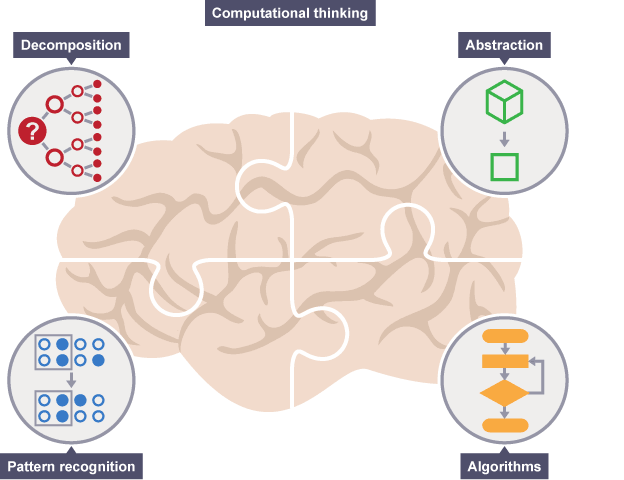
\includegraphics[scale=0.3]{large.png} 
\end{center}
\caption{Fonte: Introduction to computational thinking \footnote{\url{https://www.bbc.co.uk/bitesize/guides/zp92mp3/revision/1}}}
\end{figure}



\end{frame}

\begin{frame}{Resolvendo problemas complexos}

\begin{itemize}

\item Divida um problema complexo em uma série de problemas pequenos e mais gerenciáveis(decomposição).
\item Encontre similaridades entre os problemas menores (reconhecimento de padrão).
\item Foque apenas nos detalhes importantes e ignore informações irrelevantes (abstração).
\item Projete a solução dos problemas menores utilizando regras simples. 
\end{itemize}

\end{frame}

%%%%%%%%%%%%%%%%%%%%%%%%%%%%%%%%%%%%%%%%%%%%%%%%%%%%%%%%%%%%%%%%%%%%

\section{Decomposição}

\begin{frame}{Decomposição}

\begin{itemize}
    \item A decomposição é o primeiro passo no processo de resolução utilizando o pensamento computacional.
    \item Um problema difícil pode ser dividido em partes mais simples que podem ser resolvido diretamente.
\end{itemize}

\end{frame}

%%%%%%%%%%%%%%%%%%%%%%%%%%%%%%%%%%%%%%%%%%%%%%%%%%%%%%%%%%%%%%%%%%%%
\begin{frame}{Decomposição}

Considere a tarefa de desenhar a seguinte figura:

\begin{center}
\begin{tikzpicture}
\draw [fill=yellow](0,0) -- (2,2) -- (1,2) -- (3,4) -- (2,4) -- (2,4) -- (4,6) -- (6,6) -- (4.1,4.1) -- (5.1,4.1) -- (3.1,2.1) -- (4.1,2.1) -- (0,0);
%\draw (3,1) -- (0,0);

\end{tikzpicture}

\end{center}

\end{frame}


%%%%%%%%%%%%%%%%%%%%%%%%%%%%%%%%%%%%%%%%%%%%%%%%%%%%%%%%%%%%%%%%%%%%
\begin{frame}{Decomposição}

O problema pode ser decomposto em desenhar 11 pequenas partes.

\begin{center}
\begin{tikzpicture}
\draw [fill=yellow, line width = 1pt,](0,0) -- (2,2) -- (1,2) -- (3,4) -- (2,4) -- (4,6) -- (6,6) -- (4.1,4.1) -- (5.1,4.1) -- (3.1,2.1) -- (4.1,2.1) -- (0,0);

\draw [draw=red, line width = 2pt,](0,0) -- (2,2);
\draw [draw=blue, line width = 2pt,](2,2) -- (1,2);
\draw [draw=olive, line width = 2pt,](1,2) -- (3,4);
\draw [draw=green, line width = 2pt,](3,4) -- (2,4);
\draw [draw=brown, line width = 2pt,](2,4) -- (4,6);
\draw [draw=violet, line width = 2pt,](4,6) -- (6,6);
\draw [draw=magenta, line width = 2pt,](6,6) -- (4.1,4.1);
\draw [draw=lime, line width = 2pt,](4.1,4.1) -- (5.1,4.1);
\draw [draw=orange, line width = 2pt,](5.1,4.1) -- (3.1,2.1);
\draw [draw=pink, line width = 2pt,](3.1,2.1) -- (4.1,2.1);
\draw [draw=cyan, line width = 2pt,](4.1,2.1) -- (0,0);





\end{tikzpicture}

\end{center}




\end{frame}

%%%%%%%%%%%%%%%%%%%%%%%%%%%%%%%%%%%%%%%%%%%%%%%%%%%%%%%%%%%%%%%%%%%%

\section{Reconhecimento de Padrão}

\begin{frame}{Reconhecimento de Padrão}

\begin{itemize}
    \item Os padrões são características e similaridades que são compartilhadas entre os subproblemas encontrados pela decomposição.
    \item Essas similaridades podem ajudar a resolver a tarefa mais complexa.
\end{itemize}
\end{frame}


%%%%%%%%%%%%%%%%%%%%%%%%%%%%%%%%%%%%%%%%%%%%%%%%%%%%%%%%%%%%%%%%%%%%

\begin{frame}{Reconhecimento de Padrão}

Podemos separar em 5 padrões diferentes.

\begin{center}
\begin{tikzpicture}
\draw [fill=yellow, line width = 1pt,](0,0) -- (2,2) -- (1,2) -- (3,4) -- (2,4) -- (4,6) -- (6,6) -- (4,4) -- (5,4) -- (3,2) -- (4,2) -- (0,0);

\draw [draw=red, line width = 2pt,](0,0) -- (2,2);
\draw [draw=blue, line width = 2pt,](2,2) -- (1,2);
\draw [draw=red, line width = 2pt,](1,2) -- (3,4);
\draw [draw=blue, line width = 2pt,](3,4) -- (2,4);
\draw [draw=red, line width = 2pt,](2,4) -- (4,6);
\draw [draw=green, line width = 2pt,](4,6) -- (6,6);
\draw [draw=brown, line width = 2pt,](6,6) -- (4,4);
\draw [draw=green, line width = 2pt,](4,4) -- (5,4);
\draw [draw=brown, line width = 2pt,](5,4) -- (3,2);
\draw [draw=green, line width = 2pt,](3,2) -- (4,2);
\draw [draw=cyan, line width = 2pt,](4,2) -- (0,0);
\end{tikzpicture}

\end{center}




\end{frame}

%%%%%%%%%%%%%%%%%%%%%%%%%%%%%%%%%%%%%%%%%%%%%%%%%%%%%%%%%%%%%%%%%%%%

\section{Abstração}

\begin{frame}{Abstração}

\begin{itemize}
    \item A abstração pode ser entendida como a definição das características mais importantes e a filtragem dos detalhes e características que não precisamos.
    \item Características gerais e detalhes para assar um bolo \footnote{https://www.bbc.co.uk/bitesize/guides/zttrcdm/revision/2}
    
    \begin{tabular}{p{5cm}p{5cm}}
    Características Gerais & Detalhes \\
    \hline
    Precisamos saber que um bolo tem ingredientes & Não precisamos saber quais são esses ingredientes\\
    \hline
    Precisamos saber que cada ingrediente tem uma quantidade especificada & Não precisamos saber qual é essa quantidade\\
    \hline 
Precisamos saber que cada bolo precisa de um tempo específico para assar & Não precisamos saber quanto tempo é o tempo\\
    \end{tabular}
    
    
    
\end{itemize}



\end{frame}

%%%%%%%%%%%%%%%%%%%%%%%%%%%%%%%%%%%%%%%%%%%%%%%%%%%%%%%%%%%%%%%%%%%%


\begin{frame}{Abstração}


A característica mais importante de cada subproblema é que todos são retas que podem ser definidas por dois pontos. 

\begin{center}
\begin{tikzpicture}
\draw [fill=yellow, line width = 1pt,](0,0) -- (2,2) -- (1,2) -- (3,4) -- (2,4) -- (4,6) -- (6,6) -- (4,4) -- (5,4) -- (3,2) -- (4,2) -- (0,0);


\end{tikzpicture}

\end{center}


\end{frame}



\begin{frame}{Abstração}

Note que a abstração é bastante importante para conseguimos resolver o problema com o auxílio do computador. Vamos colocar a nossa imagem no plano cartesiano.

\begin{center}
\begin{tikzpicture}
\draw [fill=yellow, line width = 1pt,](0,0) -- (2,2) -- (1,2) -- (3,4) -- (2,4) -- (4,6) -- (6,6) -- (4,4) -- (5,4) -- (3,2) -- (4,2) -- (0,0);

\draw[step=1cm] (0,0) grid (6,6);

\end{tikzpicture}

\end{center}


\end{frame}

\section{Algoritmo}

\begin{frame}{Algoritmo}

\begin{itemize}
    \item Um algoritmo é um plano passo a passo para resolver um problema.
    \item Em um algoritmo, cada instrução é identificada e a ordem em que devem ser executadas é definida. 
    \item Os algoritmos são frequentemente usados como ponto de partida para a criação de um programa de computador e, às vezes, são escritos como um fluxograma ou em pseudocódigo. 
\end{itemize}



\end{frame}

%%%%%%%%%%%%%%%%%%%%%%%%%%%%%%%%%%%%%%%%%%%%%%%%%%%%%%%%%%%%%%%%%%%%


\begin{frame}{Algoritmo em pseudocódigo}


\begin{algorithm}[H]
\caption{Desenhando Figura}
\begin{algorithmic}
\State Desenhe um traço diagonal 2 unidades para cima;
\State Desenhe um traço para a esquerda de 1 unidade;
\State Desenhe uma traço diagonal 2 unidades para cima;
\State Desenhe um traço para a esquerda de 1 unidade;
\State Desenhe uma traço diagonal 2 unidades para cima;
\State Desenhe um traço a direita 2 unidade;
\State Desenhe uma traço diagonal 2 unidades para baixo;
\State Desenhe um traço para a direita de 1 unidade;
\State Desenhe uma traço diagonal 2 unidades para baixo;
\State Desenhe um traço para a direita de 1 unidade;
\State Desenhe uma traço para o ponto inicial;
\end{algorithmic}
\end{algorithm}

\end{frame}



\begin{frame}{Algoritmo}

\begin{itemize}
    \item Note que o algoritmo apresenta as instruções e a ordem em que as instruções devem ser executadas.
   
   \item Lembrando que o algoritmo é independente da linguagem. A implementação do algoritmo em uma linguagem específica depende dos recursos disponíveis na linguagem
   
   \item Vamos mostrar como esse algoritmo usando a linguagem Scratch
   
   
    

    
    
\end{itemize}

\end{frame}

%%%%%%%%%%%%%%%%%%%%%%%%%%%%%%%%%%%%%%%%%%%%%%%%%%%%%%%%%%%%%%%%%%%%






\begin{frame}[fragile]{Algoritmo utilizando a linguagem Scratch}

\begin{figure}
\begin{center}
	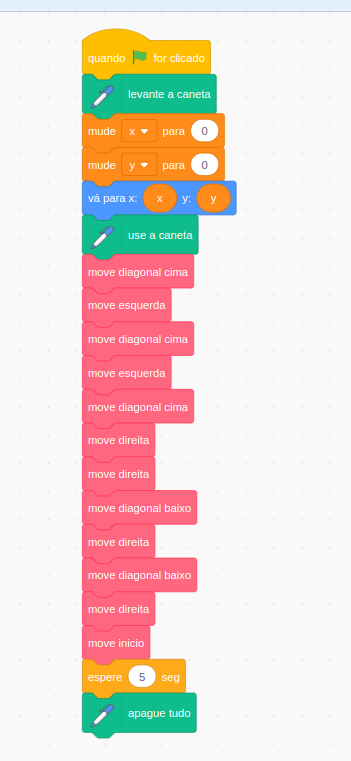
\includegraphics[scale=0.3]{Raio.png} 
\end{center}
\end{figure}

\end{frame}


\begin{frame}[fragile]{Algoritmo utilizando a linguagem Scratch}

\begin{figure}
\begin{center}
	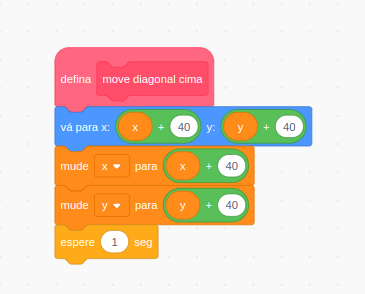
\includegraphics[scale=0.5]{diagonal cima.png} 
\end{center}
\end{figure}

\end{frame}




\section{Sequência Didática Sugerida}

\begin{frame}{Sequência Didática}

\begin{itemize}
    \item Uma sequência didática é um encadeamento de passos ligados entre si parar tornar mais eficiente o processo de aprendizagem.

\item As sequências didáticas são planejadas e desenvolvidas para a realização de determinados objetivos educacionais.

\item Vamos considerar que a sequência didática deve apresentar os objetivos, público-alvo, conteúdo, tempo para execução da atividade, Recursos Necessários e o detalhamento da atividade em passos.
\end{itemize}    

\end{frame}


\begin{frame}{Sequência Didática}

\begin{itemize}
\item \textbf{Objetivos:} Desenvolver a criatividade, resolução de problemas e o pensamento computacional.

\item \textbf{Público-alvo:}  Alunos a partir do primeiro ano do Ensino Médio.

\item \textbf{Conteúdo:} Decomposição, Reconhecimento de Padrão e Algoritmo.

\item \textbf{Tempo:} 30 minutos

\item \textbf{Recursos:} Quadro e pincel

\item \textbf{Recursos opcionais:} Computador com o Scratch instalado.
\end{itemize}
    
\end{frame}

\begin{frame}{Sequência Didática}

\begin{itemize}
\item \textbf{Passo 1:} Apresentação da atividade

Nesse passo, o professor apresenta a figura que será desenhada. O professor pode separar a sala de aula em equipes. Cada equipe deve criar uma descrição de uma sequência de passos que será executada por um outro aluno no quadro da outra equipe  que deve ficar com os olhos fechados ou uma venda. 

\item \textbf{Passo 2:} Execução da sequência de instrução

Nesse passo, o professor vai avaliar a execução da sequência de instruções. O aluno que está executando deve seguir as instruções que foram criadas pela outra equipe. 


\end{itemize}
    
\end{frame}


\begin{frame}{Sequência Didática}

\begin{itemize}
    \item \textbf{Passo 3:} Avaliação da sequência de instrução

Nesse passo, os alunos devem avaliar todos os algoritmos apresentados por todas equipes. Destacando os pontos fracos e fortes de cada solução.


\item \textbf{Passo 4:} Utilizando o scratch

Nesse passo, os alunos serão desafiados a tentarem transpor seu algoritmo para a linguagem Scratch.

\item \textbf{Passo 5:} Avaliação

A avaliação deve levar a conta a fase de construção e execução da sequência de instruções.

\end{itemize}    
    
\end{frame}



% \section{Encontrando o maior}

% \begin{frame}{Tarefa}

% \begin{itemize}

% \item Dado um conjunto de valores, encontre o maior dos valores.

% \begin{center}
% \begin{tabular}{|c|c|c|c|c|}
% \hline
% 10    &  15 & 30 & 42 & 14 \\
% \hline
% \end{tabular}
% \end{center}

% \item Você pode dizer que esse problema é muito fácil e a resposta claramente é 42. 

% \item Como você resolveria esse problema com os olhos fechados e podendo fazer perguntas simples para uma outra pessoa.

% \end{itemize}


% \end{frame}



% \begin{frame}{Decomposição}

% \begin{itemize}

% \item Sabemos que a resposta é o elemento que é maior que todos os outros.

% \item Nesse problema, precisaremos guardar uma informação que chamaremos de candidato, utilizaremos o candidato para comparar com cada um dos valores do nosso conjunto.

% \item Possivelmente, esse candidato pode ser desbancado por um dos valores do nosso conjunto e terá que ser atualizado.


% \end{itemize}


% \end{frame}


% \begin{frame}{Decomposição}


% \begin{tikzpicture}
% \node[rectangle, draw] (problema) at (0,0){Encontrar o maior elemento do conjunto};
% \node[rectangle, draw] (candidato) at (0,-1) {Selecionar um 
% candidato inicial};
% \node[rectangle, draw] (teste) at (1,-3) {Testar se o elemento $i$ desbanca o candidato e atualizar o candidato}; 
% \draw[->]  (problema) -- (candidato);
% \draw[->]  (problema) -- (teste);

% \end{tikzpicture}



% \end{frame}


% \begin{frame}{Reconhecimento de Padrões}


% \begin{itemize}
%     \item O subproblema de testar se um elemento desbanca o candidato atual e atualiza o candidato atual é o mesmo subproblema para todos os elementos do conjunto.
%     \item O que pode mudar entre os testes para cada elemento é que o candidato pode ter sido atualizado.
% \end{itemize}


% \end{frame}


% \begin{frame}{Abstração}


% \begin{itemize}
%     \item Os valores podem ser armazenados em um vetor e podem ser acessados por um índice começado por 1 até o tamanho do conjunto.
%     \item Para realizar o teste e atualização, precisamos acessar o elemento a ser testado e do candidato atual.
% \end{itemize}


% \end{frame}

% \begin{frame}{Algoritmo em pseudocódigo}


% \begin{algorithm}[H]
% \caption{maior\_elemento(A)}
% \begin{algorithmic}
% \Require o tamanho do vetor A deve ser maior que 1.
% \Ensure Devolve o maior elemento do vetor

% \State $candidato \gets A[1]$
% \State $n \gets tamanho(A)$

% \For{$i \gets 1$ \textbf{até} $n$}

% \If{A[i] > candidato}
% \State $candidato \gets A[i]$
% \EndIf

% \EndFor

% \State \Return A[i]

% \end{algorithmic}
% \end{algorithm}

% \end{frame}

% \begin{frame}[fragile]{Algoritmo utilizando a linguagem Python}

% \begin{minted}{Python}[H]
% def maior_elemento(A):
% 	candidato = A[0]
% 	n = len(A)
% 	for i in range(n):
% 		if A[i] > candidato:
% 			candidato = A[i]
% 	return candidato
% if __name__ == "__main__":
% 	print( maior_elemento([4,10,42,15,30]))	

% \end{minted}

% \end{frame}

\end{document}